\documentclass[tikz]{standalone}

\colorlet{FilledSurface}{blue!20}
\colorlet{FilledSurfaceGroupOne}{blue!20}
\colorlet{FilledSurfaceGroupTwo}{red!20}
\colorlet{FilledSurfaceGroupThree}{green!20}
\colorlet{FilledSurfaceGroupFour}{magenta!20}
\colorlet{FormulaBackground}{green!10}
\colorlet{FormulaFrame}{green}


\usetikzlibrary{calc, angles}

\begin{document}
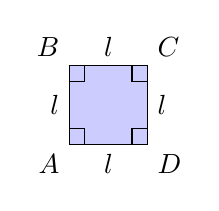
\begin{tikzpicture}

\coordinate (A) at (0, 0);
\coordinate (B) at (0, 1);
\coordinate (C) at (1, 1);
\coordinate (D) at (1, 0);
\draw[fill = FilledSurfaceGroupOne]
    (A) node[below left]{$A$}
    -- node[left] {$l$} (B) node[above left]{$B$}
    -- node[above] {$l$} (C) node[above right]{$C$}
    -- node[right] {$l$} (D) node[below right]{$D$}
    -- node[below] {$l$} cycle;

\path pic [draw,angle radius=2mm] {right angle = A--B--C};
\path pic [draw,angle radius=2mm] {right angle = B--C--D};
\path pic [draw,angle radius=2mm] {right angle = C--D--A};
\path pic [draw,angle radius=2mm] {right angle = D--A--B};

\end{tikzpicture}
\end{document}
